\documentclass[11pt]{article}
\usepackage[a4paper,margin=2.2cm]{geometry}
\usepackage{booktabs,graphicx,tabularx,array,caption,amsmath,float,placeins,microtype}
\usepackage[hidelinks]{hyperref}
\captionsetup{font=small,labelfont=bf,skip=4pt}
\newcolumntype{L}{>{\raggedright\arraybackslash}X}
\setlength{\tabcolsep}{4pt}
\newcommand{\tabnote}[1]{\par\vspace{3pt}\footnotesize\emph{Notes:} #1\normalsize}
\newcommand{\prov}[1]{\textsf{\footnotesize[#1]}}
\newcommand{\qRows}{2629}\newcommand{\qOkTot}{99.8}\newcommand{\qOkDisp}{93.5}\newcommand{\qKeys}{377}\newcommand{\qKeysNine}{180}\newcommand{\qKeysSeven}{233}\newcommand{\qKeysOne}{68}
\newcommand{\bTopTen}{84}\newcommand{\bNauthTwentyThree}{277}
\input{b3_stats.tex}\newcommand{\bSevenMatched}{132}\newcommand{\bSevenTotal}{176}\newcommand{\bSevenAllHOD}{279}\newcommand{\bSevenUnRecv}{92}
\newcommand{\bEightYear}{2023-24}

\title{What the state told us about itself\\[2pt]\large The data received in the RTI audit, by provenance}
\author{Amar Priyadarshi\thanks{For Gaurav Sood. Generated by \texttt{reports/report2\_received\_data/analysis.py} in the \texttt{rti-responses} repository. Nothing here conditions on treatment arm.}}
\date{25 September 2026}
\begin{document}
\maketitle

\section*{Three kinds of data}
Every table carries a provenance tag. \prov{A} is a document a public information officer enclosed with a reply to our request. \prov{B} is a public document at a website a reply pointed to instead of supplying the information: the Tamil Nadu State Information Commission's annual reports (cited by the Agriculture Secretariat, TN-052) and the Central Information Commission's annual reports (cited by the Directorate of Family Welfare, TN-308). \prov{C} is the same kind of publication sought by us for states without replies; Maharashtra's reports are downloaded and deferred, and the Karnataka and Telangana commission sites are unreachable from outside India. Type B is analytically the strongest: official, covering every authority whether or not it answered us, and predating our filings.

\begin{table}[H]\centering\small
\caption{Coverage and parse quality of the commission data \prov{B}}
\begin{tabularx}{\textwidth}{lL}\toprule
Tamil Nadu SIC, 2015--2023 & Per-authority annexure, 21 fields (requests, transfers, replies, rejections by clause, pending, charges, first appeals). \qRows\ authority-year rows after dropping department totals. Names harmonised across years into \qKeys\ authorities, of which \qKeysNine\ appear in all nine years and \qKeysSeven\ in seven or more; \qKeysOne\ appear once (renamed, merged, or truncated by the PDF). Row checks: total $=$ opening $+$ received holds for \qOkTot\% of rows; total $=$ replied $+$ transferred $+$ rejected $+$ pending holds for \qOkDisp\% (failures are mostly blank pending cells). The 2019--2022 reports print the table rotated, and a few names are truncated. \\
Central IC, 2020-21 to 2023-24 & Annexure 1, one column per public authority; the ``UT of Delhi'' block holds 190--200 authorities a year. The 2024-25 report is a scanned image and is not parsed. \\
\bottomrule\end{tabularx}
\end{table}

\section{Tamil Nadu, 2015 to 2023 \prov{B}}
\begin{table}[H]\centering\small
\caption{State-level RTI activity as reported by public authorities to the commission}
\footnotesize\begin{tabular}{lrrrrrrr}\toprule
Year & Authorities & Received & Transf. (\%) & Replied (\%) & Rejected (\%) & FA (\%) & Charges/req (Rs) \\\midrule
\csname @@input\endcsname tab_b1.tex 
\bottomrule\end{tabular}
\tabnote{Sums over authority rows; shares are ratios of sums to requests received. ``Replied'' is the commission's ``disposed by giving information''. First appeals are those received by first appellate authorities in the year. Charges are copying and other charges collected, excluding the Rs~10 application fee where separately reported. 2021 is the first full year of the online portal, which coincides with the jump in volume.}
\end{table}
\begin{figure}[H]\centering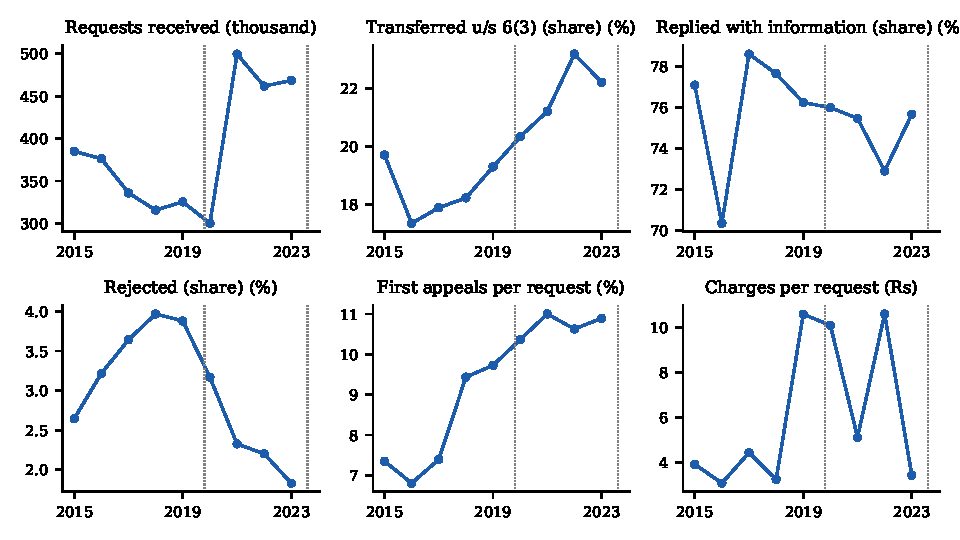
\includegraphics{fig_b1.pdf}
\caption{The same series, with the 2019 amendment and the DPDP Act marked}
\tabnote{Annual data; the amendment (October 2019) and COVID (2020) are adjacent, so nothing here separates them.}
\end{figure}

\begin{table}[H]\centering\small
\caption{Departments ranked by 2023 volume}
\footnotesize\begin{tabularx}{\textwidth}{Lrrrrrrr}\toprule
Department & Auth. & Received & Share (\%) & Transf. (\%) & Replied (\%) & Rejected (\%) & FA (\%) \\\midrule
\csname @@input\endcsname tab_b2.tex 
\bottomrule\end{tabularx}
\tabnote{Top 15 of 40 departments in 2023. Department assignment follows the report's own grouping. The top 10 percent of authorities (\bNauthTwentyThree\ in 2023) handle \bTopTen\ percent of requests (Figure~\ref{fig:conc}).}
\end{table}
\begin{figure}[H]\centering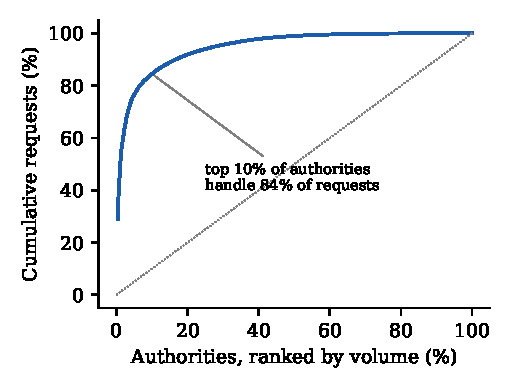
\includegraphics{fig_b2.pdf}\caption{Concentration of request volume across authorities, 2023}\label{fig:conc}\end{figure}

\begin{table}[H]\centering\small
\caption{Tier as a routing layer: pooled 2015--2023}
\footnotesize\begin{tabular}{lrrrrrrr}\toprule
Tier & Auth. & Received/yr & Transf. (\%) & Replied (\%) & Rejected (\%) & Req./PIO & FA (\%) \\\midrule
\csname @@input\endcsname tab_b4.tex 
\bottomrule\end{tabular}
\tabnote{Tier from the authority's name: ``Secretariat'' departments; heads of department (directorates and commissionerates); corporations, boards, commissions, universities and tribunals. A secretariat department routes about two thirds of what it receives under Section~6(3). This is the basis for the proposed PAP amendment that a transfer at the secretariat tier is scored as the compliant response it is.}
\end{table}

\begin{table}[H]\centering\small
\caption{Persistence of authority behaviour: two-way fixed effects, authorities with five or more years}
\footnotesize\begin{tabular}{lrrrr}\toprule
Outcome & Authorities & Rows & Between-authority $R^2$ & Lag-1 autocorr. \\\midrule
\csname @@input\endcsname tab_b3.tex 
\bottomrule\end{tabular}
\tabnote{Specification: $y_{it} = \alpha_i + \gamma_t + \varepsilon_{it}$. ``Between-authority $R^2$'' is the increase in $R^2$ from adding authority effects to year effects. Lag-1 autocorrelation is the correlation of $y_{it}$ with $y_{i,t-1}$ over consecutive years. Volume is almost entirely an authority characteristic; the reply share is about half persistent; the appeal rate is mostly year-to-year noise. Implication for the audit: request volume is a strong pre-treatment covariate, and an office's official reply share is a meaningful, if noisy, prior for its behaviour toward us.}
\end{table}
\begin{figure}[H]\centering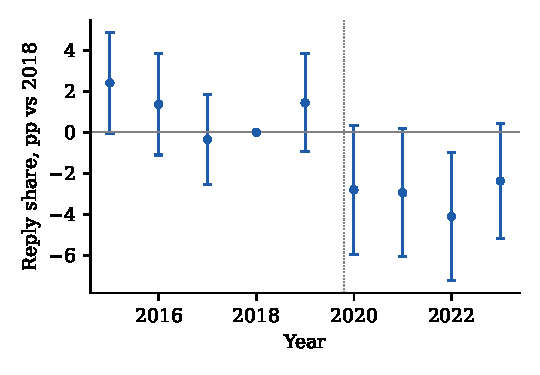
\includegraphics{fig_b3.pdf}
\caption{Year effects on the reply share, 2018 base, authority fixed effects, 95\% intervals clustered by authority (\bThreeN\ authorities)}
\tabnote{An event-study reading around the 2019 amendment is confounded by COVID and by the 2021 portal launch; the figure is descriptive.}
\end{figure}

\begin{table}[H]\centering\footnotesize
\caption{The appeals funnel}
\scriptsize\begin{tabular}{lrrrrrrrr}\toprule
Year & Requests & First appeals & FA/req (\%) & FA disposed & FA rejected & FA pending & 2nd appeals (SIC) & SIC disposed \\\midrule
\csname @@input\endcsname tab_b5.tex 
\bottomrule\end{tabular}
\tabnote{First-appeal columns from the authority annexes; second-appeal columns from the body of the 2023 report (21,476 received, 8,369 disposed). The 2023 annexure does not report first appeals rejected or pending. The commission disposes well under half of what it receives in a year, which is the ``silent commission'' outcome for the appeals estimand.}
\end{table}

\section{The audit sample in the official record \prov{B}}
\begin{table}[H]\centering\small
\caption{Matching the Tamil Nadu batch's department and head-of-department offices to commission rows}
\footnotesize\begin{tabular}{lrrrrrr}\toprule
Tier & Sampled & Matched & Match (\%) & Median req./yr & Median replied (\%) & Median transf. (\%) \\\midrule
\csname @@input\endcsname tab_b7.tex 
\bottomrule\end{tabular}
\tabnote{Fuzzy matching of office names to harmonised commission authorities, using 2021--2023 means; cutoff 0.75 with manual review pending for unmatched offices. Sub-offices (824 of the 1,000) are not itemised in the annexes; their department aggregate is. The matched file (\texttt{data/tn\_sample\_commission\_covariates.csv}) supplies the pre-treatment covariates proposed for the pre-analysis plan: log request volume, transfer share, and official reply share. Unmatched head-of-department offices in the commission list (\bSevenAllHOD\ in total) have a median of \bSevenUnRecv\ requests a year.}
\end{table}

\section{What the replies enclosed \prov{A}}
\begin{table}[H]\centering\small
\caption{One office measured three ways: Co-operation, Food and Consumer Protection Secretariat}
\footnotesize\begin{tabularx}{\textwidth}{lLlrrrr}\toprule
Period & Source & Basis & Received & Transferred & Replied & First appeals \\\midrule
\csname @@input\endcsname tab_a1.tex 
\bottomrule\end{tabularx}
\tabnote{The register letter counts requests from August 2025 to July 2026; the enclosed return and the commission rows are calendar years. The 2019 row fails the disposal identity (a rotated-table misalignment) and the 2015 row lacks a transfer figure; both are flagged in the parse log. The office's own return for 2025 (502) sits below its commission-reported 2022 and 2023 figures and well below the 712 it reports for the following twelve months, which is the first case for the register-versus-return cross-check the design promises.}
\end{table}
\begin{figure}[H]\centering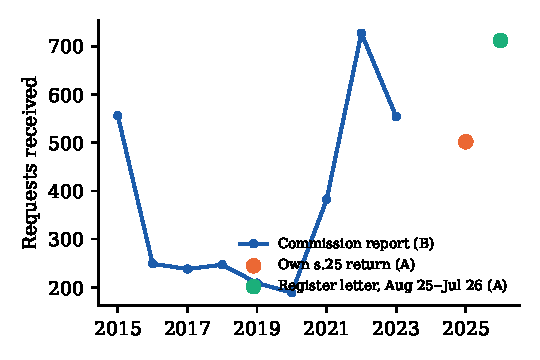
\includegraphics{fig_a1.pdf}\caption{Requests received by the Co-operation Secretariat, by source}\end{figure}

\begin{table}[H]\centering\footnotesize
\caption{Section 25(2) Format I return for 2025, enclosed by the Co-operation Secretariat (TN-173)}
\begin{tabularx}{\textwidth}{Lrrrrrrr}\toprule
Public authority & PIOs & Received & Transf. (\%) & Replied (\%) & Rejected (\%) & FA (\%) & Rs/req. \\\midrule
\csname @@input\endcsname tab_a2.tex 
\bottomrule\end{tabularx}
\tabnote{Transcribed from the scanned enclosure. The Civil Supplies CID rejects almost everything under Section~24 (exempt organisation), a lawful blanket exemption. One penalty (Rs~15,000) was imposed against about 8,400 requests. ``Rs/request'' is application fees plus charges collected per request received.}
\end{table}
\begin{table}[H]\centering\small
\caption{The same authorities in the commission's 2023 report versus their own 2025 return}
\footnotesize\begin{tabularx}{\textwidth}{Lrrrr}\toprule
Authority & Recd 2023 \prov{B} & Recd 2025 \prov{A} & Replied 2023 (\%) & Replied 2025 (\%) \\\midrule
\csname @@input\endcsname tab_a2b.tex 
\bottomrule\end{tabularx}
\end{table}

\begin{table}[H]\centering\scriptsize
\caption{Register extracts and count tables enclosed in replies}
\begin{tabularx}{\textwidth}{lp{3.4cm}lp{2.1cm}rrrL}\toprule
ID & Authority & Format & Period & Received & Transf. & Replied & Notes \\\midrule
\csname @@input\endcsname tab_a3.tex 
\bottomrule\end{tabularx}
\tabnote{Format A is one row per application in the office's register; B is monthly or category counts; C is period totals. Entry of the two fee-pending registers (TN-173, 416~pp; TN-283, 69~pp) follows payment. The Kannada register (KA-057) awaits transcription.}
\end{table}

\section{Delhi benchmark \prov{B}}
\begin{table}[H]\centering\small
\caption{UT of Delhi public authorities in the Central Information Commission's annexes}
\scriptsize\begin{tabular}{lrrrrrrrr}\toprule
Year & Auth. & Received & Transf. (\%) & Replied (\%) & Rejected (\%) & FA (\%) & Rs/req. & Penalties (Rs) \\\midrule
\csname @@input\endcsname tab_b8.tex 
\bottomrule\end{tabular}
\tabnote{Authorities reporting online annual returns under the Delhi block; columns where a year's layout differs are left as reported and flagged in the parse log. The Delhi filings in the audit (22 drawn, 6 filed) are benchmarked against this block.}
\end{table}
\begin{table}[H]\centering\small
\caption{Largest Delhi authorities by requests, \bEightYear}
\footnotesize\begin{tabularx}{\textwidth}{Lrrrrr}\toprule
Authority & Received & Transf. (\%) & Replied (\%) & Rejected (\%) & FA (\%) \\\midrule
\csname @@input\endcsname tab_b8b.tex 
\bottomrule\end{tabularx}
\end{table}

\section*{What this changes in the pre-analysis plan}
Three amendments follow. First, tier enters as a routing layer: a Section~6(3) transfer at the secretariat tier is the modal compliant response (two thirds of what secretariats receive) and is scored as such. Second, request volume, transfer share and official reply share from the commission annexes enter as pre-treatment covariates for every matched Tamil Nadu department and head-of-department office; volume is almost entirely an authority fixed effect, so it is the natural heterogeneity dimension. Third, the office-paired misreporting estimator is specified against the official reply share for matched offices, with no selection on response on the official side.
\end{document}
